\chapter{ТЕСТИРОВАНИЕ И ОЦЕНКА ПРОИЗВОДИТЕЛЬНОСТИ СИСТЕМЫ}

В данной главе представлено описание методологии тестирования разработанного распределённого хранилища. Оценка программного комплекса разделена на два этапа: логическую верификацию гарантий безопасности (корректность поведения в штатных и аварийных ситуациях) и количественный анализ производительности системы при различных топологиях и профилях нагрузки. По постановке и характеру проверок методология близка к подходам семейства Jepsen для анализа безопасности распределённых систем \cite{jepsen}.

\section{Эмуляция сетевых аномалий}

Достоверное тестирование алгоритмов консенсуса в реальных сетевых средах сопряжено с проблемой недетерминированности: физическое оборудование и операционные системы вносят непредсказуемые задержки, что делает невозможным надежное воспроизведение сложных краевых случаев (например, одновременного отказа узлов или частичного разделения сети). 

Для решения этой проблемы в рамках программного комплекса был спроектирован и реализован специализированный инструмент — внутрипроцессный эмулятор сети. Эмулятор функционирует как прокси-слой, перехватывающий все вызовы удалённых процедур (RPC) между узлами кластера до их фактической сериализации и отправки.

Фундаментом эмулятора является глобальная матрица связности. Она представляет собой потокобезопасную структуру данных, описывающую разрешенные маршруты передачи пакетов между любыми двумя узлами $i$ и $j$. Интеграция данного компонента с тестовым фреймворком языка программирования Go позволяет реализовать методологию внедрения сбоев:

\begin{enumerate}
    \item Программная изоляция узлов. Изменяя значения в матрице связности в процессе выполнения теста, эмулятор имитирует глухой разрыв сети для выбранного узла, мгновенно отклоняя все исходящие и входящие пакеты. Это позволяет моделировать сценарии изоляции лидера и разделения кластера на изолированные сегменты.
    \item Искусственные задержки. Эмулятор способен вносить контролируемые временные задержки в доставку сообщений, провоцируя срабатывание тайм-аутов алгоритма выбора лидера.
\end{enumerate}

Использование программного эмулятора обеспечивает полную детерминированность экспериментов. Тесты выполняются локально в многопоточной среде, не зависят от внешних факторов и гарантируют стопроцентную воспроизводимость результатов.

\section{Верификация алгоритмической корректности}

Для подтверждения соответствия реализации математической модели алгоритма Raft был разработан набор автоматизированных интеграционных тестов. Проверки осуществляются посредством активного опроса состояний с заданными тайм-аутами, что исключает нестабильность тестов, характерную для методов жесткого ожидания по времени.

Все эксперименты в данном разделе проводились на базовой топологии, состоящей из трех узлов. В ходе верификации были успешно пройдены следующие критические сценарии.

\subsection{Отказ и восстановление узла}

Целью данного теста является подтверждение способности системы к автоматической ресинхронизации данных после временного аппаратного сбоя или сетевой изоляции участника.

Ход эксперимента:
\begin{enumerate}
    \item В стабильно работающем кластере эмулятор принудительно обрывает все связи для одного из узлов-последователей.
    \item На оставшемся кворуме (2 узла) координатор принимает и успешно фиксирует серию клиентских команд на модификацию данных.
    \item Изолированный узел возвращается в сеть.
\end{enumerate}

Результаты мониторинга показали, что при восстановлении связи восстановленный узел корректно обрабатывает входящий запрос \texttt{AppendEntries}. Узел обнаруживает расхождение в индексах журнала, отбрасывает невалидные данные (если таковые имеются) и реплицирует недостающий фрагмент истории от действующего лидера. По завершении фазы синхронизации состояния локальных автоматов на всех трех машинах становятся абсолютно идентичными.

\begin{figure}[H]
	\center{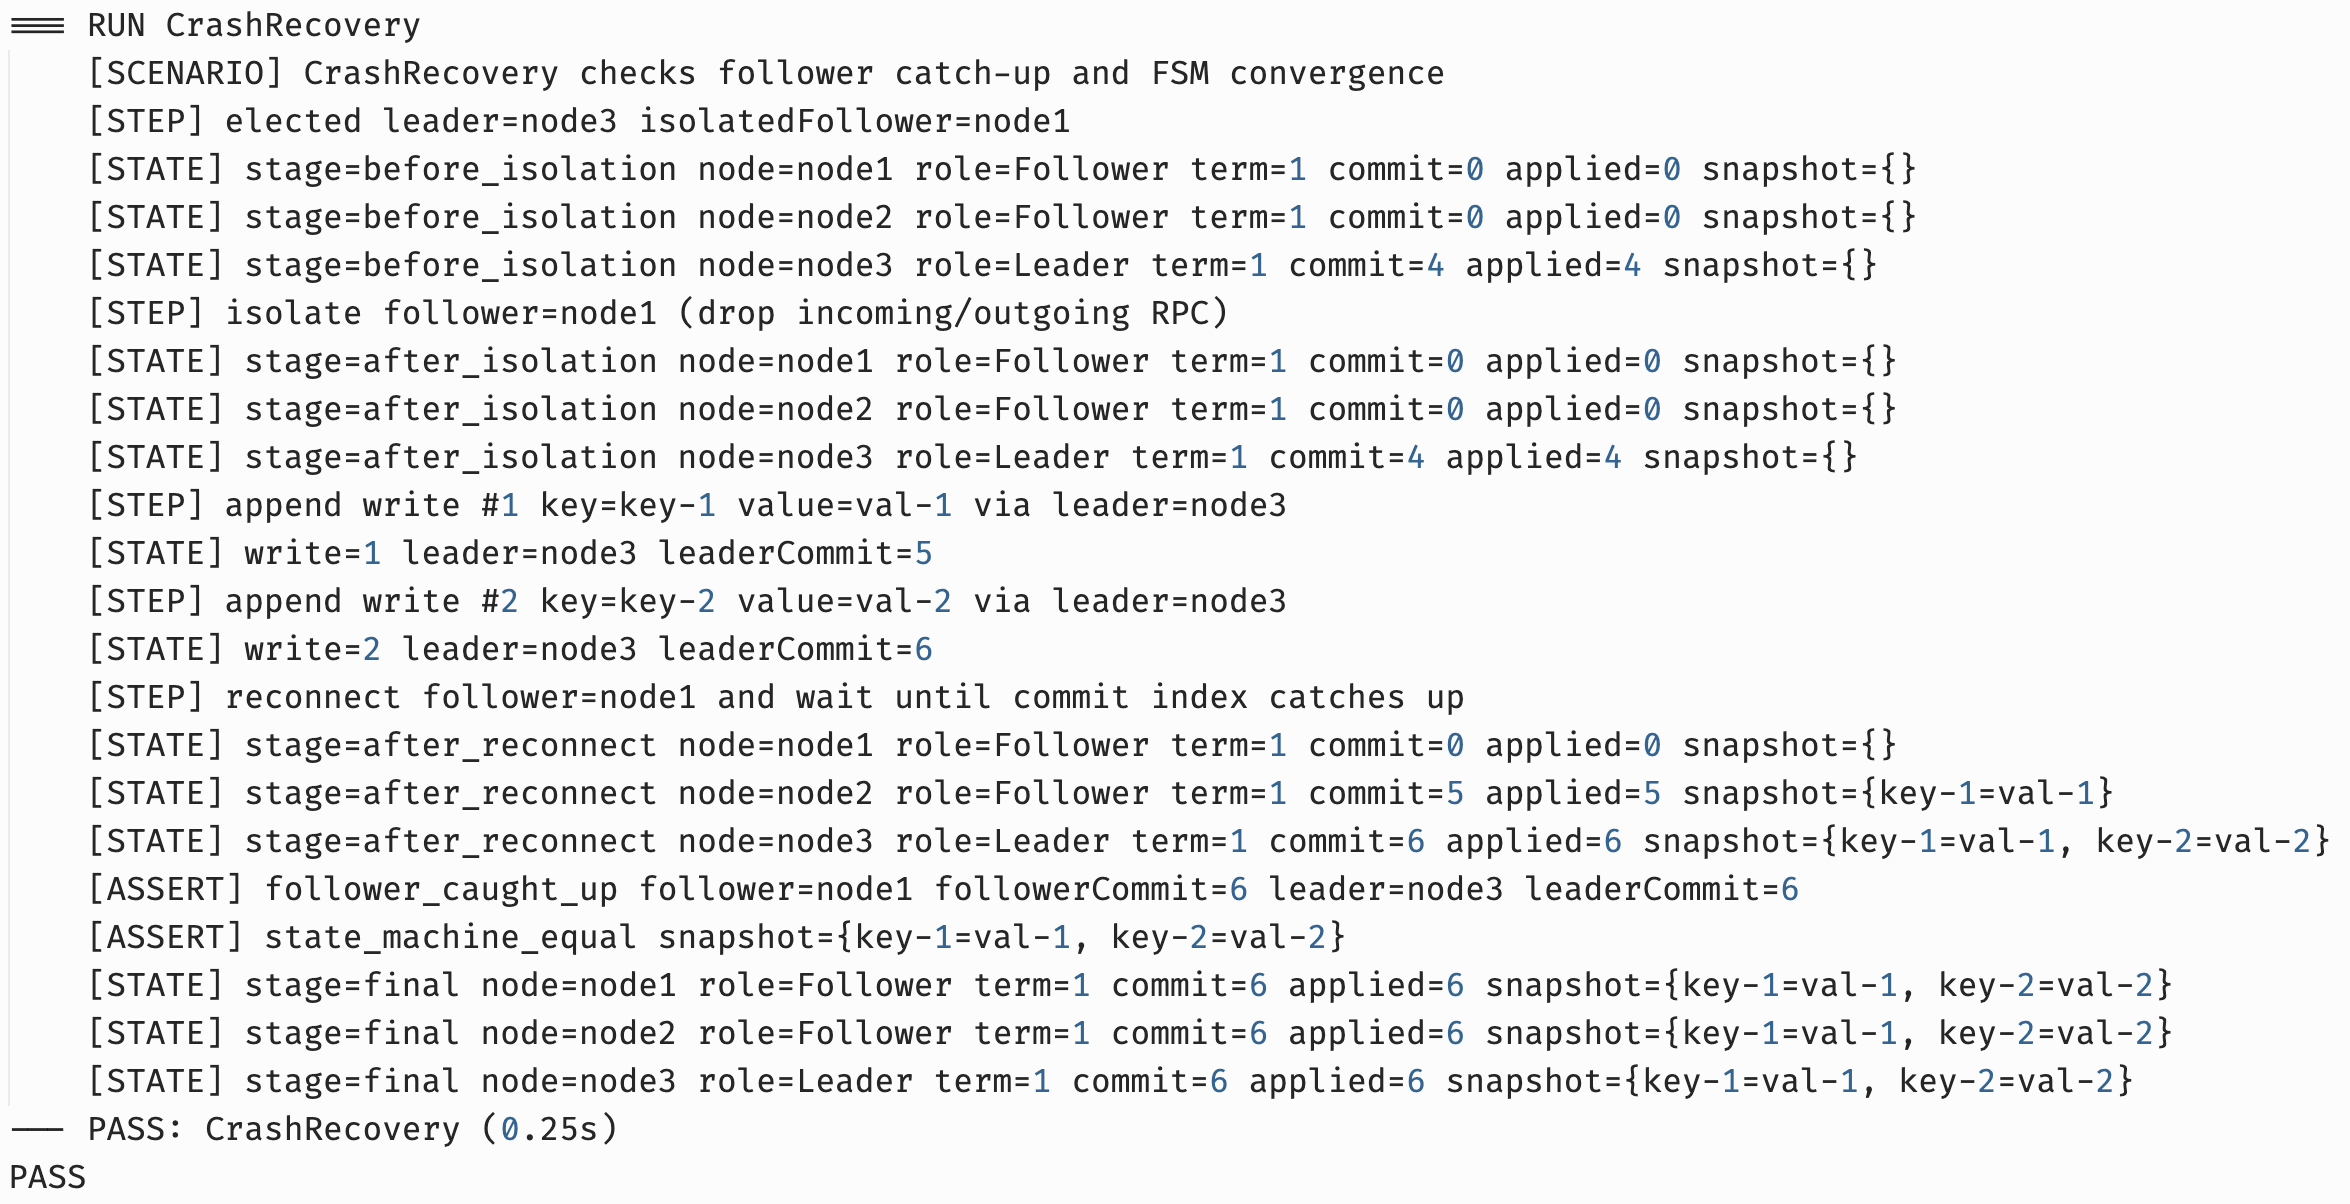
\includegraphics[width=0.9\linewidth]{images/tests/CrashRecovery.png}}
	\caption{Журнал событий: отказ и восстановление узла}
	\label{fig:crash_recovery}
\end{figure}

\subsection{Защита от фантомных чтений при раздвоении управления}

Данный сценарий критически важен для верификации свойства линеаризуемости при возникновении ситуации раздвоения управления (Split-Brain).

Ход эксперимента:
\begin{enumerate}
    \item Действующий лидер (Узел 1) изолируется от остальных участников (Узлы 2 и 3).
    \item Узлы 2 и 3, не получая сигналов активности, инициируют выборы и назначают Узел 2 новым координатором. Клиент отправляет команду записи Узлу 2, и она успешно фиксируется новым кворумом.
    \item Инициируется конкурентный запрос на чтение модифицированных данных, принудительно маршрутизированный на изолированный Узел 1.
\end{enumerate}

Результат: изолированный Узел 1 не возвращает устаревшее значение из своей оперативной памяти. В соответствии с реализованным механизмом барьера чтения, он переходит в режим ожидания подтверждений статуса лидера от большинства. Поскольку узел находится в изоляции, кворум не собирается, и запрос на чтение отклоняется по истечении тайм-аута. Тест доказывает устойчивость архитектуры к чтению неактуальных данных.

\begin{figure}[H]
	\center{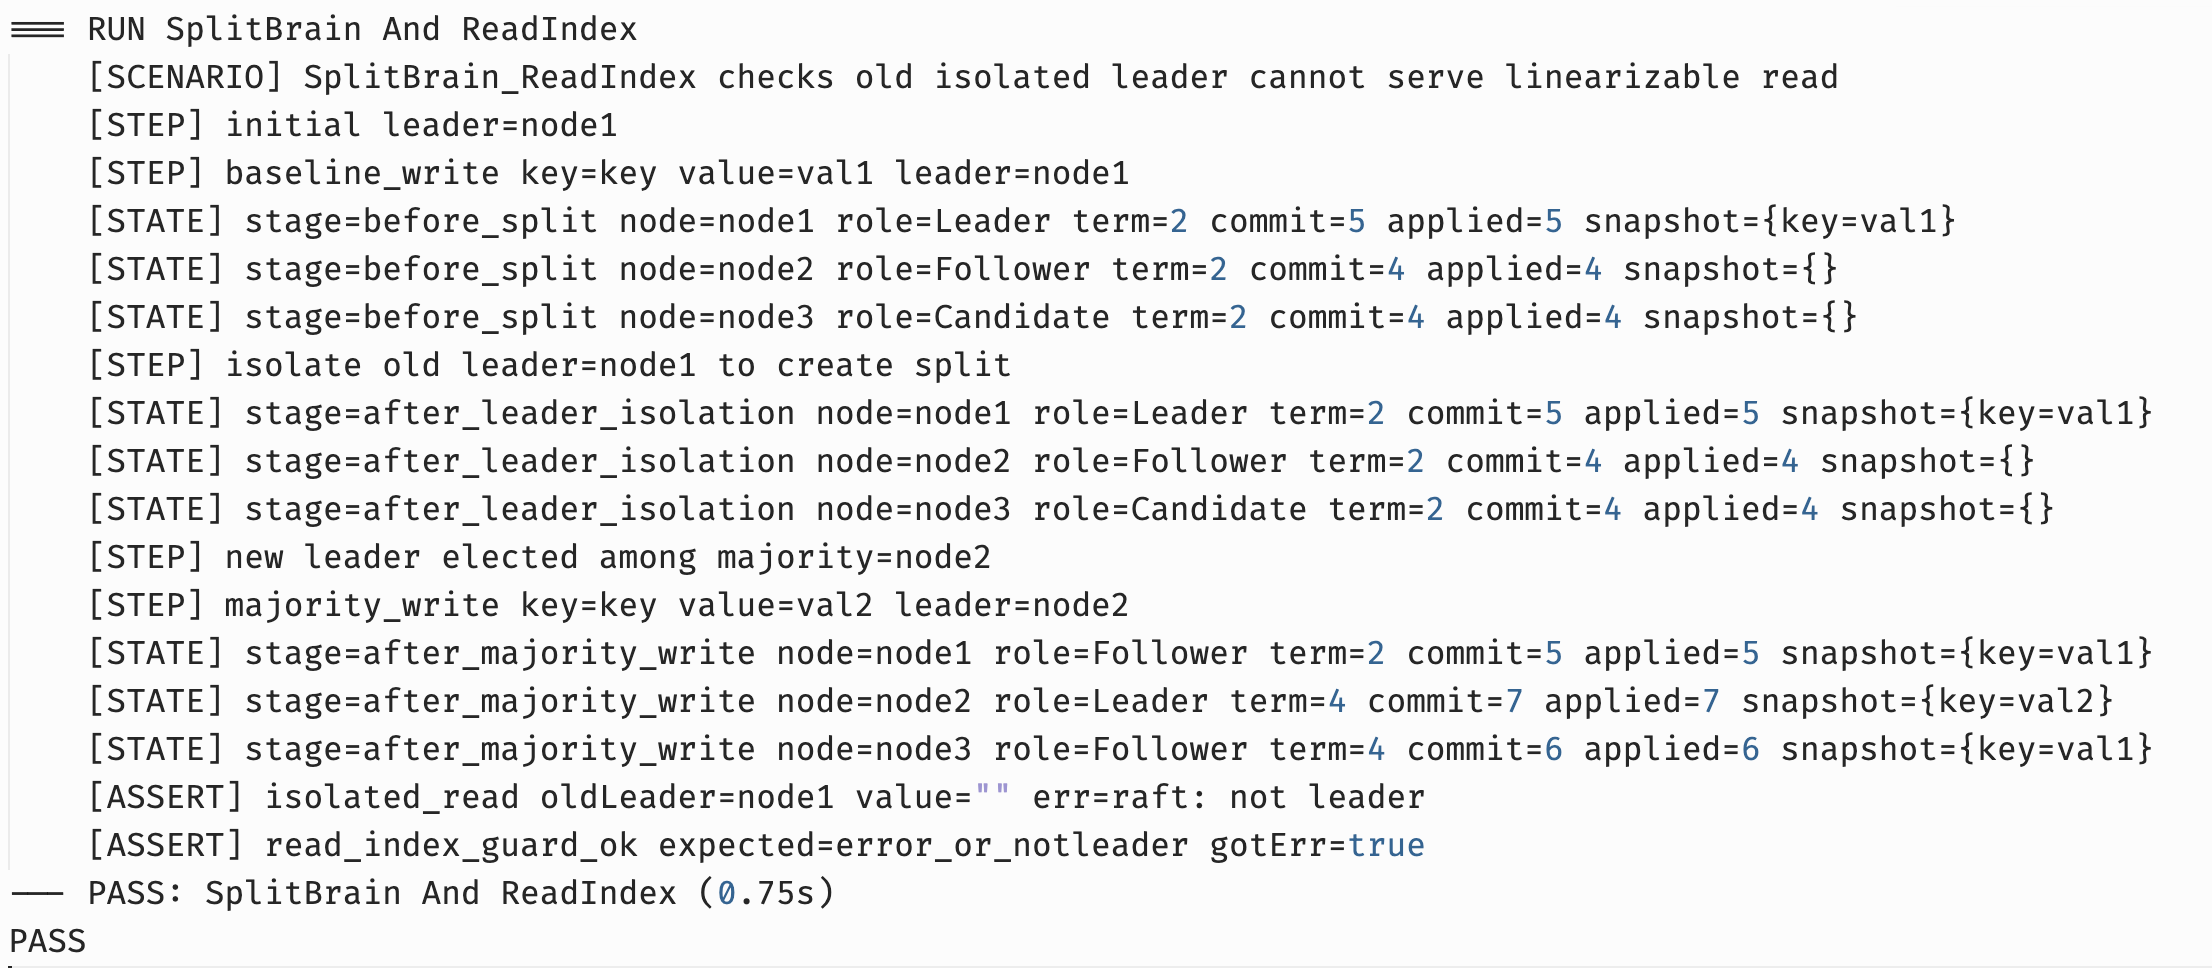
\includegraphics[width=0.9\linewidth]{images/tests/SplitBrainReads.png}}
	\caption{Журнал событий: запрос на чтение на изолированном узле}
	\label{fig:split_brain_reads}
\end{figure}

\subsection{Стресс-тестирование конкурентных транзакций}

Для проверки надежности механизма строгой сериализации запросов был смоделирован сценарий агрессивной конкурентной нагрузки. 

Ход эксперимента:
В системе инициируется 50 независимых клиентских процессов (вычислительных потоков). Каждый клиент одновременно отправляет лидеру команду инкремента одного и того же счетчика в глобальном хранилище. 

Результат: несмотря на массивный поток одновременных вызовов к сетевому интерфейсу координатора, все транзакции были выстроены алгоритмом Raft в строгую линейную последовательность в реплицированном журнале. Итоговое значение счетчика в машине состояний после завершения всех вызовов в точности составило 50. Отсутствие отклонений в меньшую или большую сторону доказывает, что механизм кворумной фиксации полностью исключает состояния гонки при параллельной модификации одних и тех же ключей.

\begin{figure}[H]
	\center{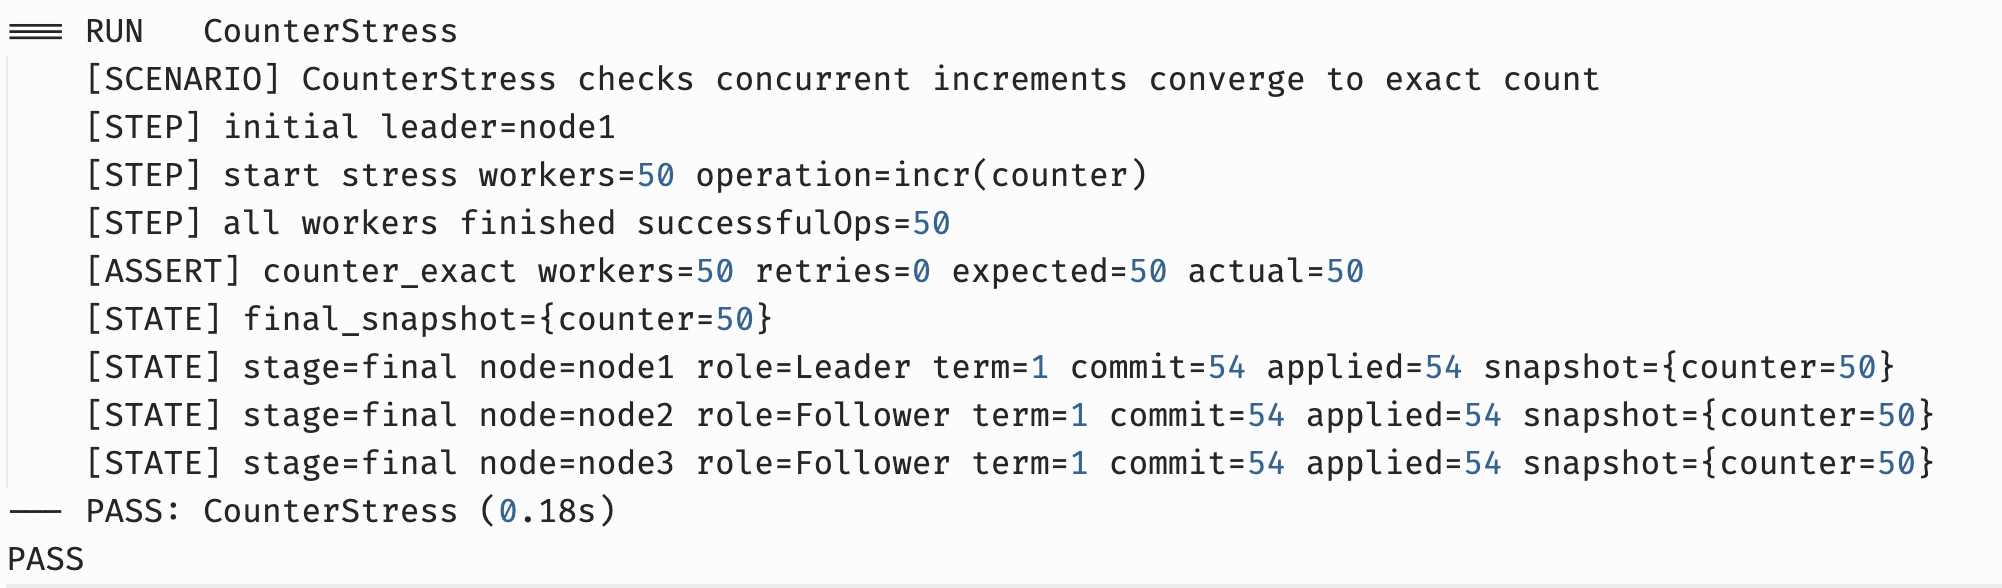
\includegraphics[width=0.9\linewidth]{images/tests/CounterStress.png}}
	\caption{Журнал событий: стресс-тестирование конкурентных транзакций}
	\label{fig:counter_stress}
\end{figure}

\section{Оценка производительности в статических конфигурациях}

Целью данного этапа экспериментального исследования является количественная оценка пропускной способности (Requests Per Second, RPS) и времени отклика (Latency) системы. Особое внимание уделяется анализу деградации производительности при масштабировании кластера «в ширину».

Для проведения замеров был разработан генератор нагрузки. В каждом эксперименте инициируется 50 независимых параллельных потоков (клиентов), которые осуществляют непрерывную отправку запросов к координатору кластера в течение фиксированного времени. 

Замеры производились для топологий размером 3, 5, 7, 11, 13 и 17 узлов. Тестирование разделено на два изолированных профиля нагрузки: интенсивная запись (100\% команд \texttt{Put}) и интенсивное чтение (100\% команд \texttt{Get}).

\subsection{Анализ производительности при модификации данных}

В сценарии интенсивной записи каждая операция требует полного цикла консенсуса: добавления команды в локальный журнал лидера, параллельной рассылки RPC-запросов \texttt{AppendEntries} всем последователям и ожидания подтверждений от строгого большинства (кворума) перед фиксацией.

\begin{figure}[H]
	\center{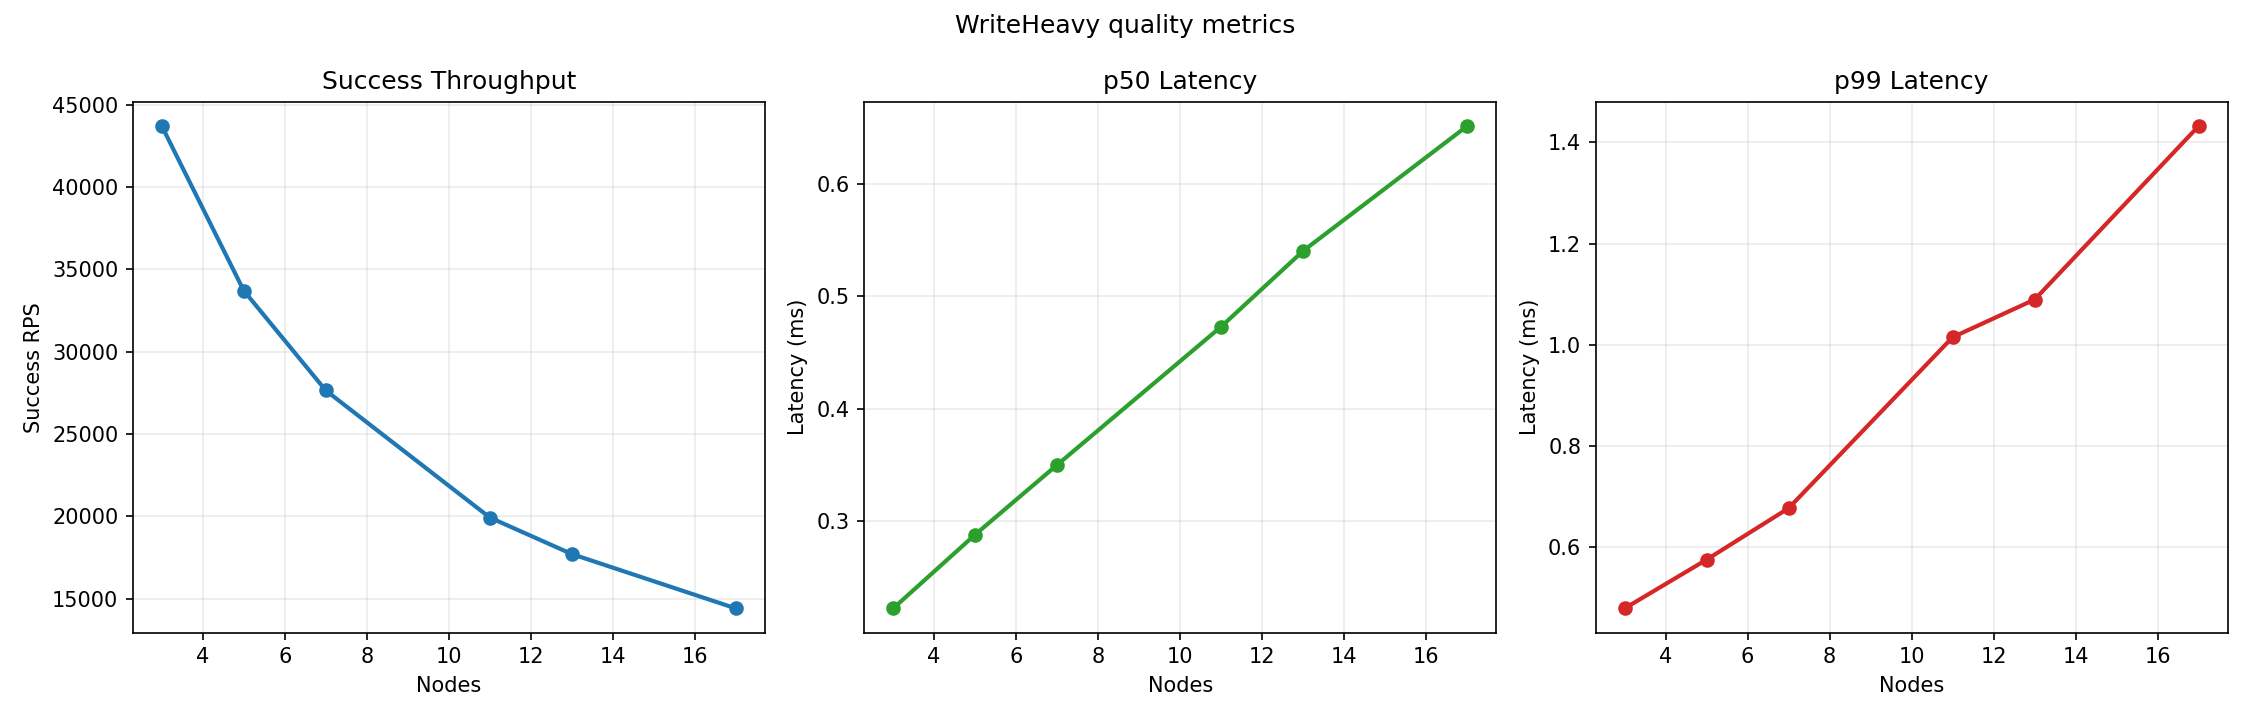
\includegraphics[width=0.9\linewidth]{images/tests/benchmark_write.png}}
	\caption{Деградация пропускной способности (RPS) и рост хвостовой задержки (p50 и p99) при масштабировании кластера (операции записи)}
	\label{fig:bench_write}
\end{figure}

Полученные данные (рис. \ref{fig:bench_write}) демонстрируют строгую обратную зависимость между размером кластера и его пропускной способностью. При переходе от минимальной отказоустойчивой конфигурации (3 узла) к расширенной (17 узлов) пропускная способность снизилась практически в 3 раза: с $\sim43\,700$ до $\sim14\,400$ RPS. 

Данная деградация математически обоснована ростом размера кворума. Для фиксации записи в кластере из 17 узлов лидер вынужден сериализовать данные для 16 последователей и ожидать ответа как минимум от 8 из них. Это многократно увеличивает нагрузку на вычислительные ресурсы координатора. Более того, ожидание ответов от большого числа машин статистически повышает вероятность влияния самого медленного узла в кворуме на общее время транзакции, что наглядно отражается в трехкратном росте хвостовой задержки (p99 увеличился с 0.47~мс до 1.43~мс).

\subsection{Анализ производительности при чтении данных}

В отличие от операций записи, профиль интенсивного чтения продемонстрировал экстраординарную стабильность. Архитектура хранилища использует барьер чтения, который позволяет возвращать данные непосредственно из оперативной памяти без записи в реплицированный журнал, но с сохранением строгой гарантии линеаризуемости.

\begin{figure}[H]
	\center{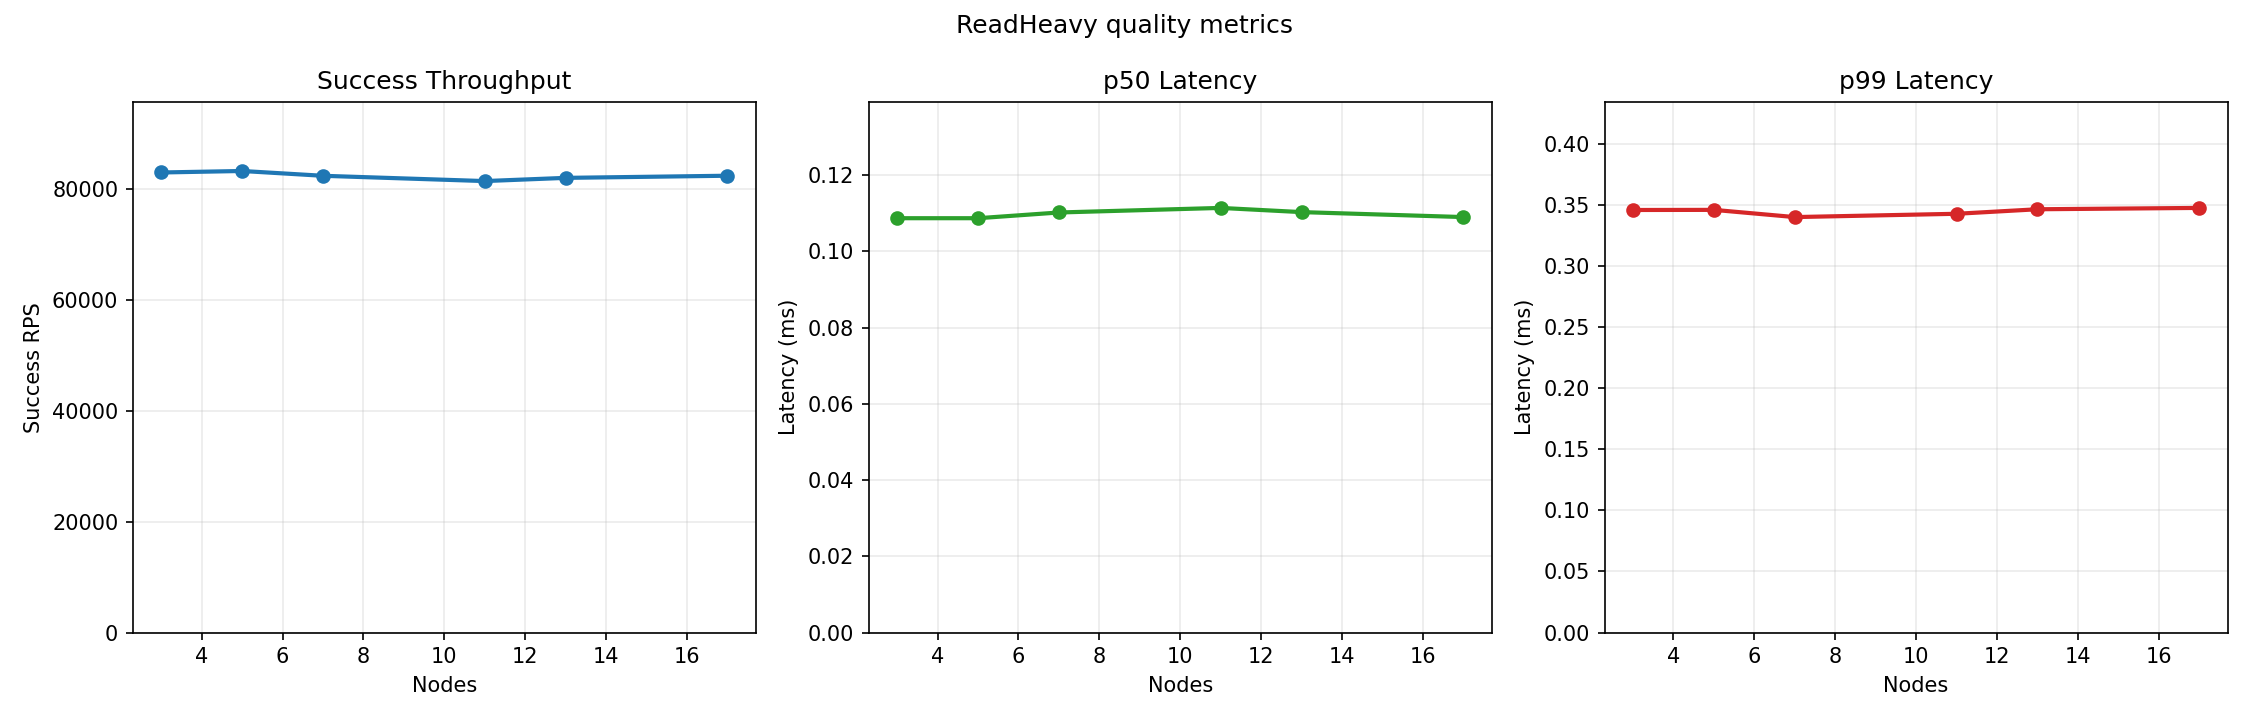
\includegraphics[width=0.9\linewidth]{images/tests/benchmark_read.png}}
	\caption{Стабильность пропускной способности (RPS) и задержки (p50 и p99) при масштабировании кластера (операции чтения)}
	\label{fig:bench_read}
\end{figure}

Данные, представленные на графике (рис. \ref{fig:bench_read}), показывают, что пропускная способность при чтении стабильно удерживается в диапазоне $81\,000 - 87\,000$ RPS независимо от количества серверов в топологии, что превосходит скорость записи в 2–6 раз. Хвостовая задержка (p99) также остается неизменной на уровне $\sim0.34$~мс.
